%%%%%%%%%%%%
%
% $Autor: Wings $
% $Datum: 2019-03-05 08:03:15Z $
% $Pfad:  Wings-hub\210520PortentaH7\PortentaH7\$
% $Name: PortentaH7$
% $Version: 4250 $
%
%%%%%%%%%%%%




\chapter{OpenMV IDE}




The OpenMV IDE is a premier integrated development environment which is a software tool  to use the openMV camera present on the Arduino vision shield.  It has a text editor ,frame buffer viewer with a histogram display and a debug terminal. It can be used across platforms, supporting Windows, Mac OS, Linux and Raspian. It was built for machine vision applications and is programmed in python\cite{OpenMV:2021}. Allerdings setzt das Werkzeug die Verwendung von MicroPython voraus. \Mynote{Prüfen, ob dies stimmt.}

\subsection{OpenMV IDE Installation}
To install the OpenMV IDE, first we need to download the IDE from their webpage \url{https://openmv.io/pages/download}.The set up file name is openmv-ide-windows-2.6.9.exe and the size of it is 1,21,573 KB. we can specify the path according to our needs. Here i have set the path as \path{C:\Users\Shoeb\AppData\Roaming\Microsoft\Windows\Start Menu\Programs\OpenMV IDE}

After the download is done,open the setup file.
Then click on Next.
\begin{figure}[H]
	\centering
	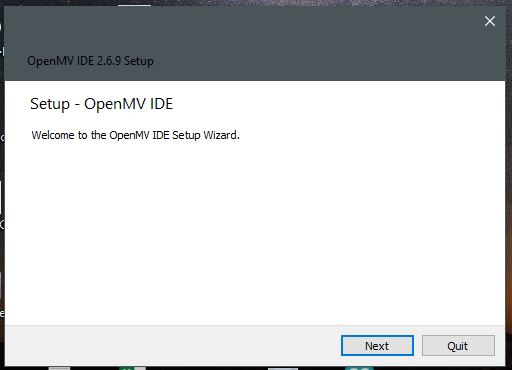
\includegraphics[width=0.8\textwidth]{Arduino/openmvins1}
	\caption{OpenMV IDE Installation}
	\label{figure 6.4}
\end{figure}

Then select the installation folder and click on Next as shown in figure \labelcref{figure 6.5}.
\begin{figure}[H]
	\centering
	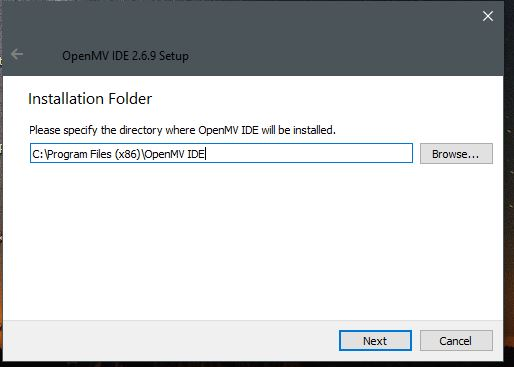
\includegraphics[width=0.8\textwidth]{Arduino/openmvins2}\
	\caption{OpenMV IDE Installation folder}
	\label{figure 6.5}
\end{figure}
Then a dialogue box pops up showing ready to install, click on Install as shown in figure \labelcref{figure 6.6}.
\begin{figure}[H]
	\centering
	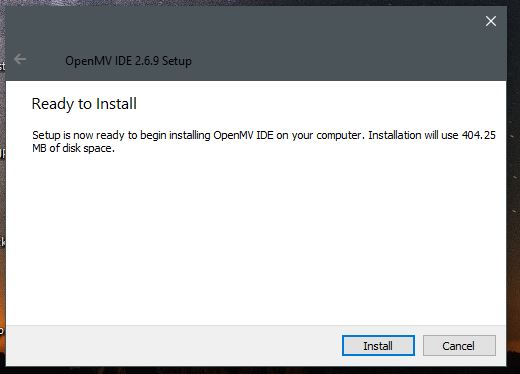
\includegraphics[width=0.8\textwidth]{Arduino/openmvins5}
	\caption{OpenMV IDE Setup Install}
	\label{figure 6.6}
\end{figure}
After the installation is done, OpenMV IDE opens up with a default program as shown in figure\labelcref{figure 6.7}.
\begin{figure}[H]
	\centering
	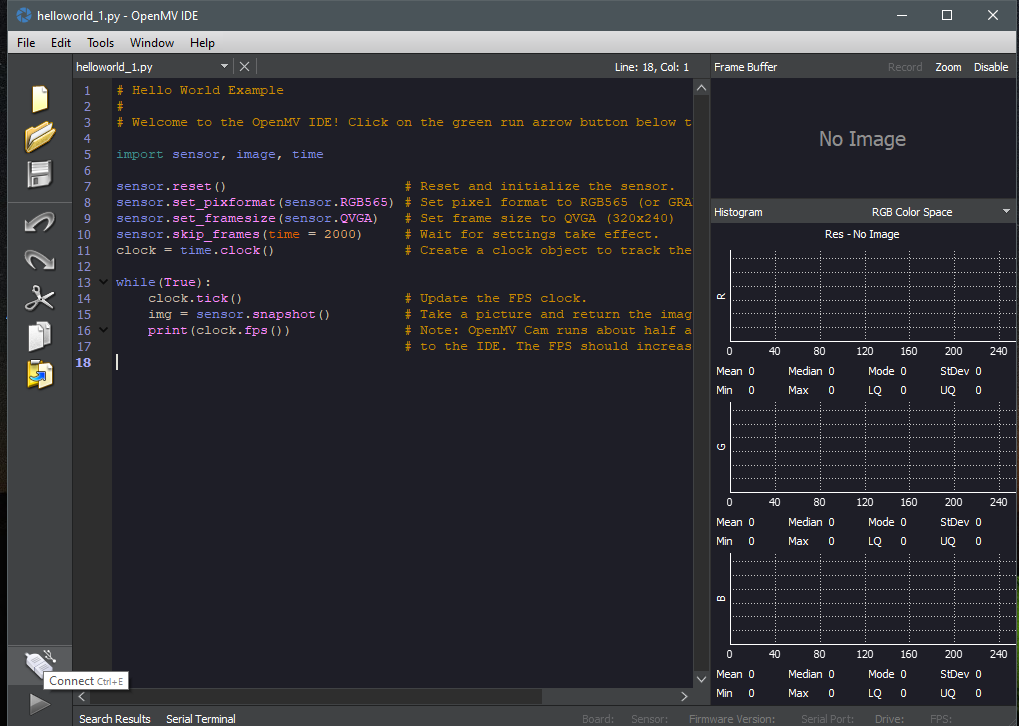
\includegraphics[width=0.8\textwidth]{Arduino/openmvide}
	\caption{OpenMV IDE}
	\label{figure 6.7}
\end{figure}


Now open the OpenMV IDE and and click on connect. Then select Install the latest release firmware(v4.0.1) and click OK as shown in figure\labelcref{figure 6.8}. 
\begin{figure}[H]
	\centering
	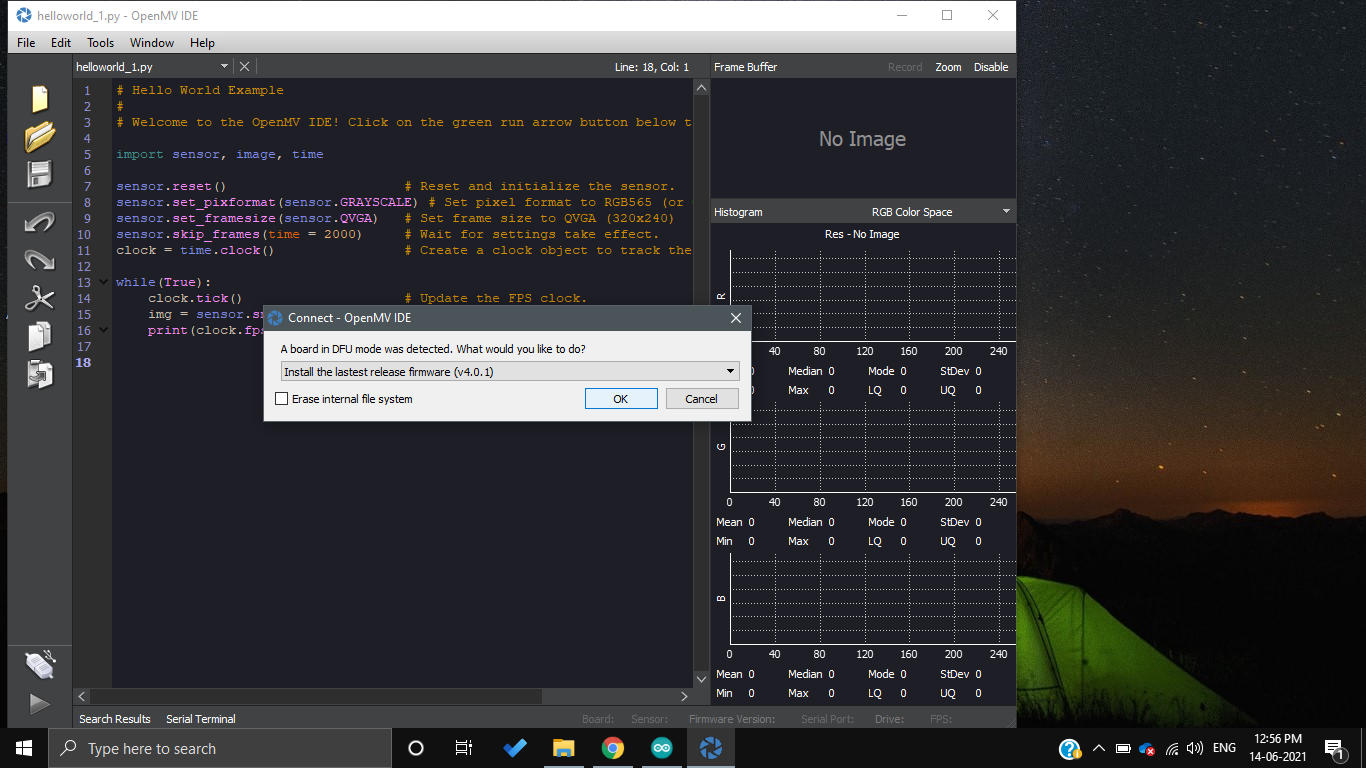
\includegraphics[width=0.8\textwidth]{Arduino/openmvinst}
	\caption{Installing latest firmware}
	\label{figure 6.8}
\end{figure}

Then a dialog box opens up saying that the update is complete as shown in figure\labelcref{figure 6.9}. 

\begin{figure}[H]
	\centering
	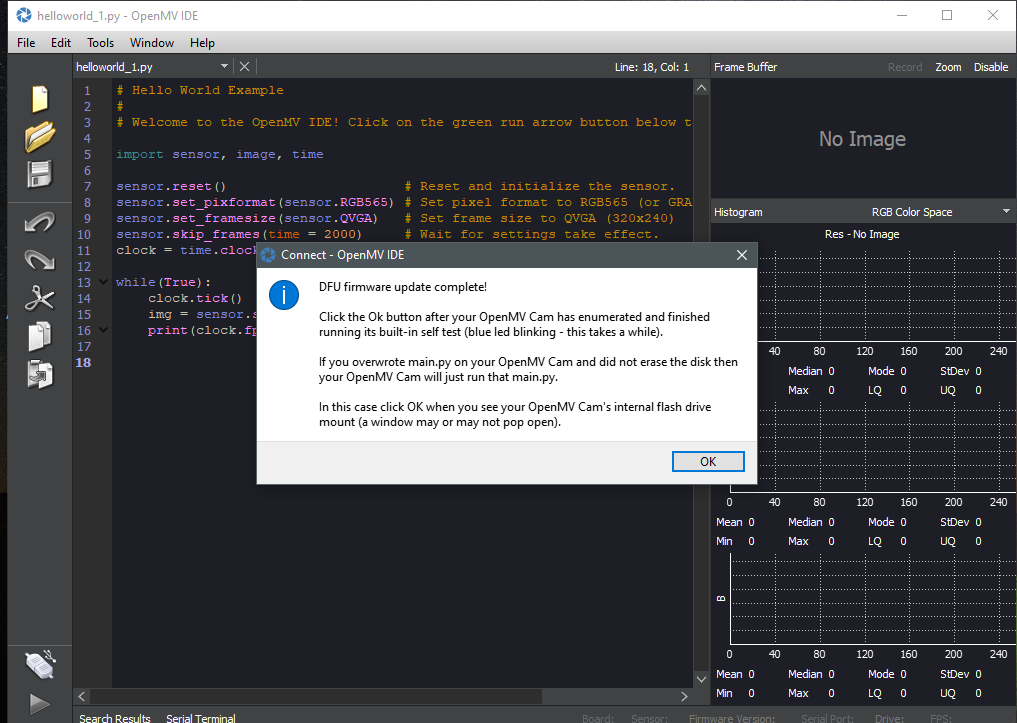
\includegraphics[width=0.8\textwidth]{Arduino/firmwareinstalled}
	\caption{firmware update complete}
	\label{figure 6.9}
\end{figure}
Now  we hit the play button to run the program. If we are not able to run then we need to reset the Arduino Portenta H7 board. After the reset is done, click on the play button at the bottom of the screen. By this, we have succesfully connected our Vision shield with Arduino Portenta H7 and now we can start doing machine vision applications using the camera provided by the Vision shield.
\subsection{OpenMV IDE Overview}
In the figure \labelcref{figure 6.9} we can see that the OpenMV IDE has an integrated frame buffer on the top right side. This lets us see the camera stream from the vision shield camera. There are 3 options on top which are record, zoom and disable.
\begin{itemize}
	\item  \textbf{Record} : This lets us record the video stream in the frame buffer at 30 FPS.
	\item \textbf{Zoom} : This option enables to zoom in or out the frame buffer viewer.
	\item \textbf{Disable} : This option lets us control the camera stream. If we disable it, then we wont be able to see th camera stream in the frame buffer. We can also save image from the frame buffer by simply right clicking it and select save as image option.
	
\end{itemize}
\textbf{Histogram Display} :
The OpenMV IDE has a histogram display which is used for getting feedback about the lighting quality in the room which is basically giving the idea about quality of the image the camera is looking at. We have four diferent options here to select such as RGB, Grayscale,YUV and LAB. These are useful in programming to determine the corect grayscale and LAB color channel settings which we need to use in the scripts.

\textbf{Serial Terminal} :
This is present at the bottom of the OpenMV IDE. All the debug text which we write in the print() command will be displayed here.

\textbf{Status Bar} :
In the status bar OpenMV IDE will display the OpenMV Cam’s Firmware Version, Serial Port, Drive, and FPS. We can also update the firmware version from here if it is not updated. The status bar displays the curent FPS, the board which is H7 in our case and the serial port label as well.

\textbf{Tools} :
In the tools, there are many options available.
\begin{itemize}
\vspace{-0.6mm}
	\item Save open script to your OpenMV cam : This lets us save the script in the OpenMV cam which is the Arduino vision shield and it will also automatically deletes comments and white spaces to save memory and it will store the script as main.py.
	\vspace{-0.6mm}
	\item Configure OpenMV cam settings file : This allow us to modify an .ini file which is stored in the OpenMV cam using OpenMV IDE which the OpenMV cam will read on bootup for particular hardware configurations.
	\vspace{-0.6mm}
	\item Reset OpenMV cam : This command resets and disconnects from the OpenMV cam.
	\vspace{-0.6mm}
\end{itemize} 






\chapter{First Steps with the Vision Shield}

\section{Introduction}

In this chapter we will be going through the installation of OpenMV IDE and the steps required for connecting the Arduino Portenta H7 with the Vision Shield using the OpenMV IDE. Further, we will be looking at the overview of the OpenMV IDE and what are the tools provided in the IDE.  Finally, we will be implementing some of the example programs provided in the OpenMV IDE.


\section{OpenMV Examples}

\subsection{Creating a basic face filter with OpenMV}

In this example we use a smiley image in portable bitmap image(.pbm) format because OpenMV supports bmp, pgm or ppm image formats and not the other image formats such as .png \cite{Romero:2020}.  This image will be overlayed on the face when it detects a face in the camera stream. 
Download the image and copy it into the flash drive.
First we load the image into a variable named as faceImage using the Image() function. We use copy\_to\_fb to false because we don?t want it to be copied automatically in to the frame buffer. Next we calculate the scale ratio to scale the bitmap image to match the detected face in the camera stream using the function \PYTHON{scale\_ratio=faceWidth/faceImage.width()}
Then we draw the bitmap image on the detected face using the function \PYTHON{draw\_image()}.
Here the face detection is done using the Haar cascade algorithm. In this algorithm, it has multiple stages in which the output of one stage gives additional information  to the input of next stage in the cascade. By doing this, it calculates the edges, lines, contrast checks in different stages and ultimately detects the face and draws a bounding box around it. 


\begin{figure}[H]
	\centering
	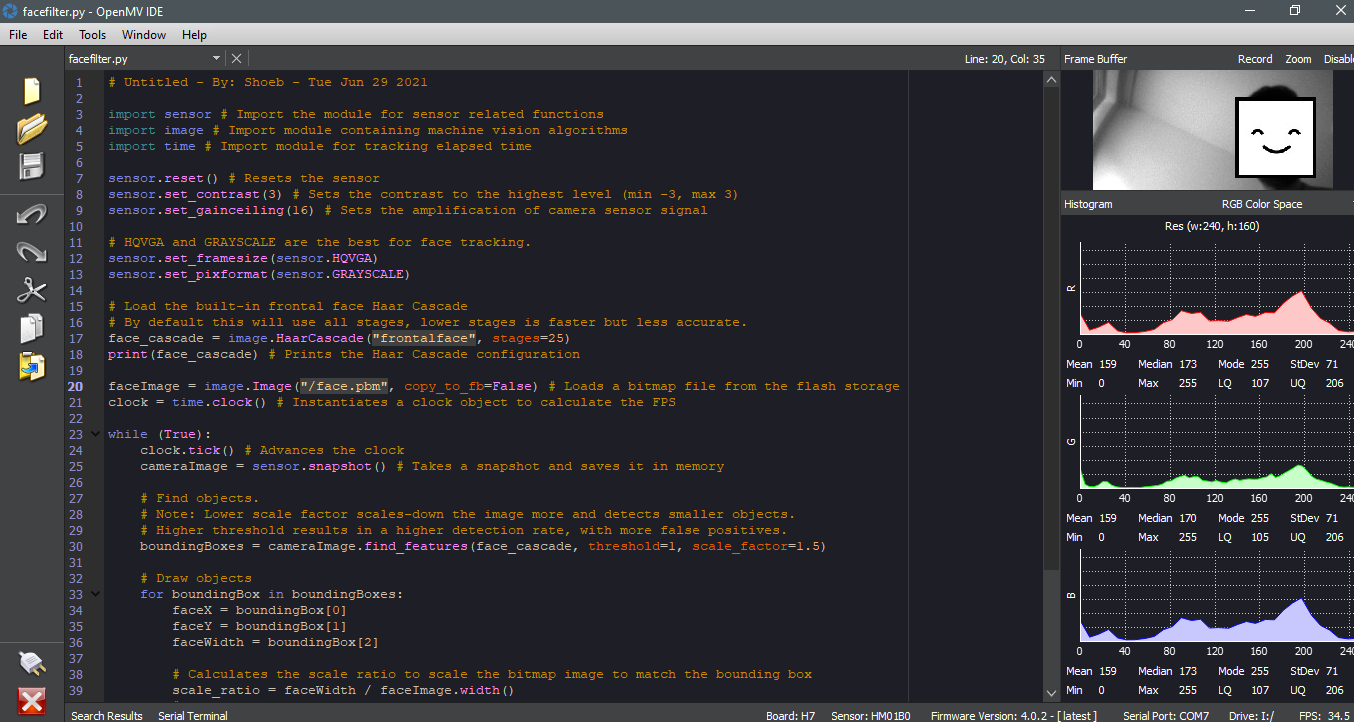
\includegraphics[width=\textwidth]{Arduino/facefilter}
	\caption{Face Filter output}
	\label{figure 6.10}
\end{figure}

As we can see from the above figure  \ref{figure 6.10} that as soon as a face is detected in the camera stream, the bitmap image which was loaded earlier is overlapped on to the detected face.

\subsection{Face tracking }

In this example, we are going to detect face and draw a bounding box around it. It uses the Haar cascade algorithm to detect faces.To do this, go to files in the OpenMV IDE and open examples and select face\_tracking. In the program, firstly, we  reset the sensor using \PYTHON{sensor.reset()} function and we  set the frame size to QVGA and set the pixel format to grayscale. Next we  load the Haar cascade using the function \PYTHON{image.HaarCascade()} . Next we  use the keypoints feature of OpenMV camera to track a face after it is detected by Haar cascade algorithm. For this, first we set the keypoints to none and when the face is detected we will use the function \PYTHON{image.find\_keypoints()} function. Then by using \PYTHON{draw\_rectangle()} function we draw a rectangle around the detected face and draw keypoints using \PYTHON{draw\_keypoints()} function. After this, we extract keypoints in the whole frame and then match this keypoints with first keypoints which was used only for face using \PYTHON{image.match\_descriptor()} function If the keypoints match is greater than 5 then we draw a rectangle around the matched feature.

\begin{figure}[H]
	\centering
	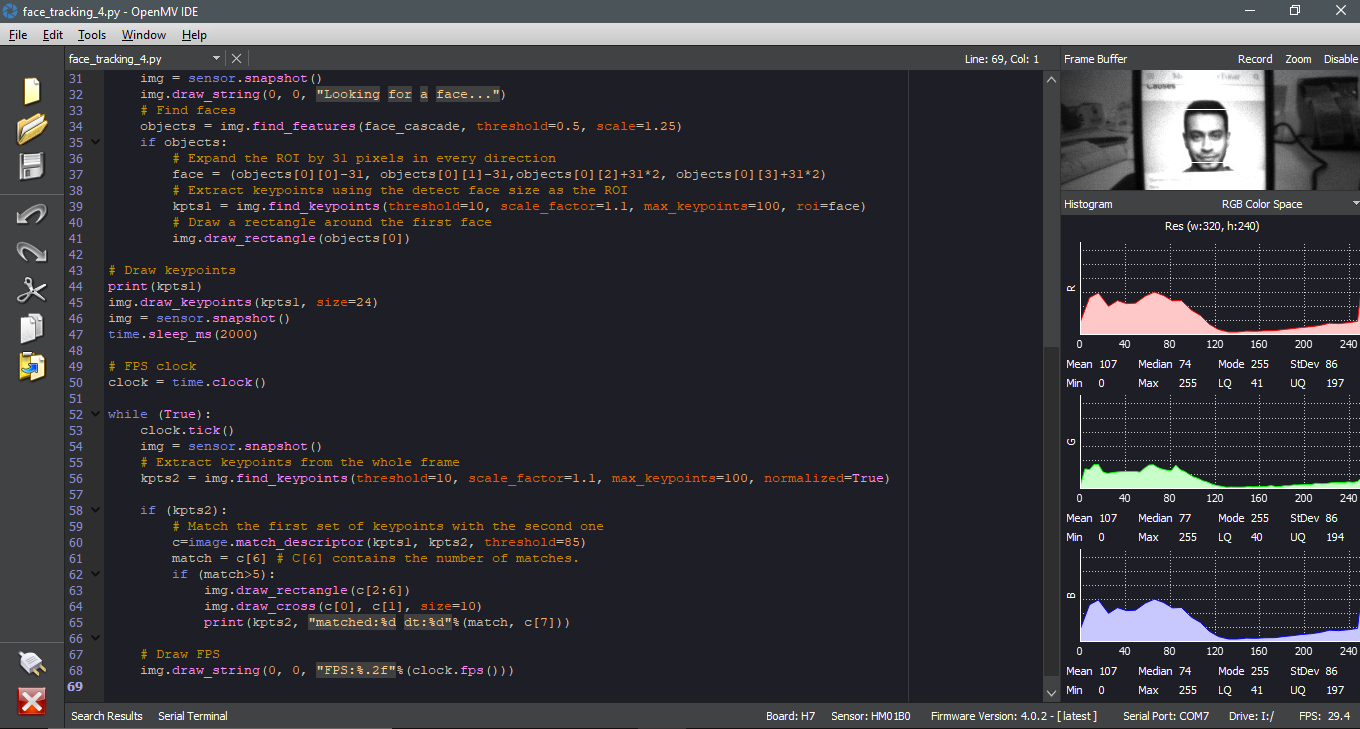
\includegraphics[width=\textwidth]{Arduino/face_tracking}
	\caption{Face tracking output}
	\label{figure 6.11}
\end{figure}

After we run this sketch, we need to point the vision shield camera towards a face and focus it properly. As soon as the face is detected in the camera stream , a rectangular box is formed around it indicating the detected face in the image. In this example, we can see that it clearly identifies the face and the bounding box is also generated around it.

\subsection{Finding circles around the objects}

In this example, we find the circles in an image using Hough transform algorithm. This algorithm is used in image processing for extracting the features such as circles or ellipses in an image.  For programming this,  we first reset the sensor as described in earlier examples. Then we take snapshot from the camera stream using \PYTHON{sensor.snapshot()} function. Then we find the circle in the image using  \PYTHON{find\_circles()} function. Lastly  we draw circles using \PYTHON{draw\_circles()} function.

\begin{figure}[H]
	\centering
	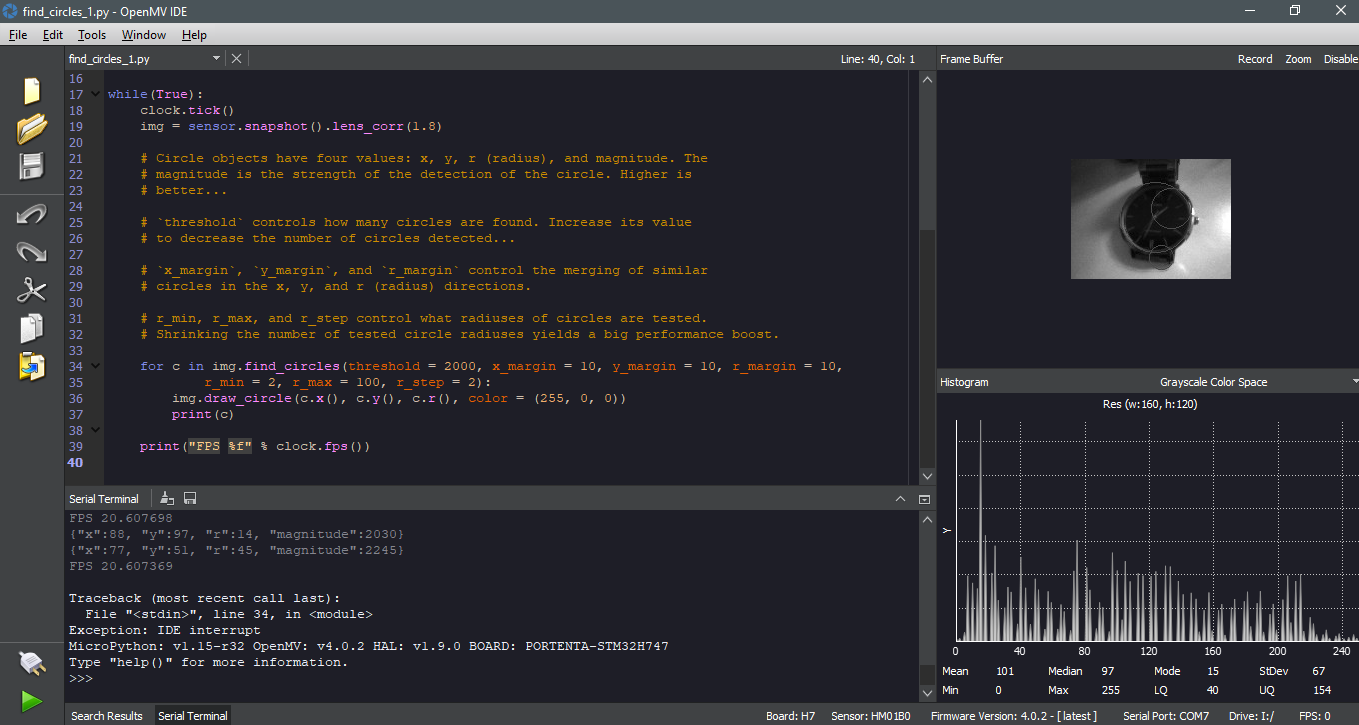
\includegraphics[width=\textwidth]{Arduino/find_circles}
	\caption{Find circles output}
	\label{figure 6.12}
\end{figure}
As can be seen from the figure \ref{figure 6.12},the ouput shows that the circles are drawn on the border of the watch. we need to bring the objects closer to the camera so that the focus is set properly in order to detect the circles around the objects.
  
\subsection{QR Code information extraction}

In this example we extract the information from QR code by using the vision shield.  This is an interesting feature of the openMV camera present in the vision shield. In order to program this, we first follow the same initialization steps as mentioned in the earlier examples.  We then take a snapshot from the camera stream using the sensor.snapshot() function and then we do the lens correction to 1.8 in order to get a better quality image using \PYTHON{lens\_corr()} function.  To extract the QR code we use \PYTHON{find\_qrcodes()} function and then we draw a rectangle around the QR code using \PYTHON{draw\_rectangle()} function.

\begin{figure}[H]
	\centering
	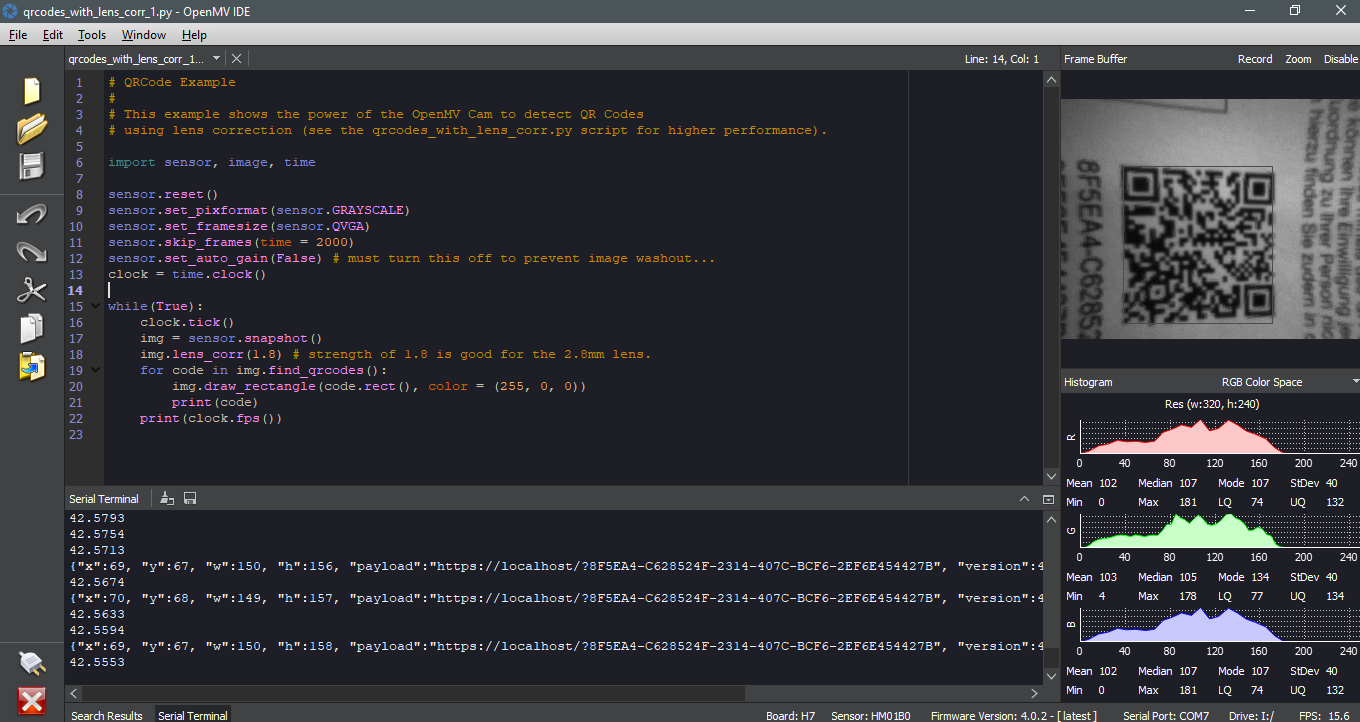
\includegraphics[width=\textwidth]{Arduino/QRcodedetection}
	\caption{QR Code output}
	\label{figure 6.13}
\end{figure}

In the output figure \ref{figure 6.13} we can see that a rectangular box is created around the QR Code and the information is extracted from it and it can be seen in the output serial terminal.



